\documentclass[a4paper,11pt,exos]{nsi} % COMPILE WITH DRAFT
\usepackage{pifont}
\usepackage{fontawesome5}
\usepackage{hyperref}



\begin{document}
\classe{\terminale Comp}
\titre{Exercices - Lois discrètes}
\maketitle

\tabularstyled[UGLiBlue]
\begin{tabular}{p{16.5cm}}
    \rowcolor{UGLiBlue}
    \ths Capacités attendues : \\

    \ding{111} Identifier des situations où une variable aléatoire suit une loi de Bernoulli, une loi binomiale ou une loi géométrique. \\
    \ding{111} Déterminer des coefficients binomiaux à l’aide du triangle de Pascal. \\
    \ding{111} Dans le cas où $X$ suit une loi binomiale, calculer à l’aide d’une calculatrice ou d’un logiciel, les probabilités des événements de type $P(X = k)$ ou $P(X \leqslant k)$, etc. Calculer explicitement ces probabilités pour une variable aléatoire suivant une loi géométrique.\\
    \ding{111} Dans le cas où $X$ suit une loi binomiale, déterminer un intervalle $I$ pour lequel la probabilité $P(X \in I )$ est inférieure à une valeur donnée $\alpha$, ou supérieure à $1 - \alpha$.\\
    \ding{111} Dans le cadre de la résolution de problème, utiliser l’espérance des lois précédentes.\\
    \ding{111} Utiliser en situation la caractérisation d’une loi géométrique par l’absence de mémoire.\\
    \ding{111} Calculer des probabilités dans des situations faisant intervenir des probabilités conditionnelles, des répétitions d’expériences aléatoires.
\end{tabular}


\vspace*{1cm}
\exo{}%Magnard p 187
\dleft{13cm}{
    Suite à des problèmes de production, un fabricant de tablettes de chocolat met en place une nouvelle chaîne de production : l'ancienne chaîne ne prend désormais en charge que 40 \% de la production.\\
    Un contrôle qualité montre que :
}
{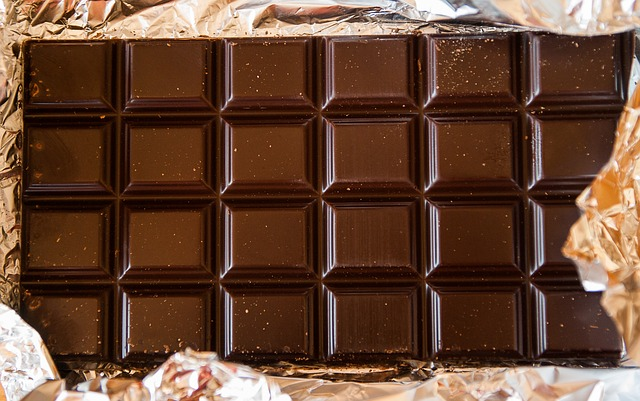
\includegraphics[width=3cm]{chocolate-1277002_640.jpg}}
\begin{enumerate}[label=\textbullet]
    \item parmi les tablettes produites par l'ancienne chaîne, 68 \% sont commercialisables ;
    \item parmi les tablettes produites par la nouvelle chaîne, 90 \% sont commercialisables.
\end{enumerate}
\begin{enumerate}
    \item Représenter la situation par un arbre pondéré.\\
    \textit{On introduira des évènements bien choisis.}
    \item Calculer la probabilité que la tablette provienne de la nouvelle chaîne et soit commercialisable.
    \item La tablette tirée au sort n'est pas commercialisable. Quelle est la probabilité qu'elle vienne de la nouvelle chaîne ?
\end{enumerate}

\newpage

\exo{ Spécificité et sensibilité d'un test}
On s'intéresse à deux test médicaux permettant de détecter des maladies.

\begin{encadrecolore}{Infos}{UGLiDarkBlue}
    \begin{enumerate}[label=\textbullet]
        \item La \textbf{sensibilité d'un test} est la probabilité que le test soit positif si la personne est porteuse de la maladie testée.
        \item La \textbf{spécificité d'un test} est la probabilité que le test soit négatif si la personne n'est pas porteuse de la maladie.
        \item La \textbf{valeur prédictive positive (VPP) d'un test} est la probabilité que la personne soit réellement malade si son test est positif.
        \item La \textbf{valeur prédictive négative (VPN) d'un test} est la probabilité que la personne ne soit pas réellement malade si son test est négatif.
    \end{enumerate}
\end{encadrecolore}

\section*{La mucoviscidose}
On s'intéresse aux patients porteurs d'une mutation dans le gène CFTR qui est impliqué dans la mucoviscidose.\\[.5em]
\dleft{13cm}{
    En France, une personne sur 34 est porteuse de la mutation (cela n'implique pas d'être malade car il s'agit d'une maladie autosomique récessive).\\
    Il existe un test pouvant détecter ces mutations avec une sensibilité de 85 \% et une spécificité proche de 100 \%.\\
}
{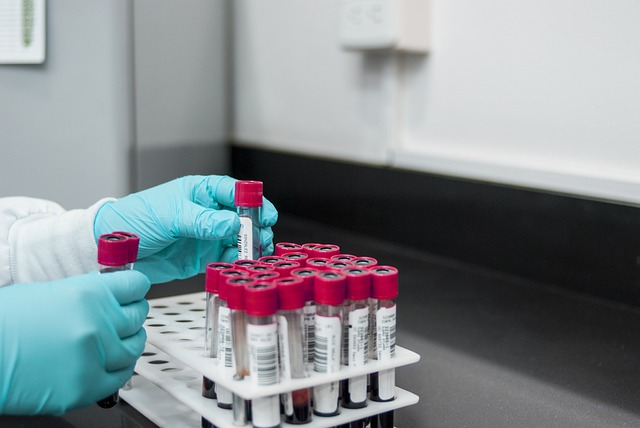
\includegraphics[width=3cm]{lab-3498584_640.jpg}}
On note :
\begin{enumerate}[label=\textbullet]
    \item M l'événement « être porteur de cette mutation » ;
    \item T l'événement « le test est positif ».
\end{enumerate}
\begin{enumerate}
    \item Traduire les probabilités de de l'énoncé à l'aide des événements T et M.
    \item A près avoir fait un test qui s'est révélé négatif, déterminer la probabilité d'être quand même porteur.
\end{enumerate}


\dleft{13cm}{
    \section*{L'appendicite}
    Pour diagnostiquer la présence d'une appendicite chez des patients présentant des douleurs abdominales aigues, on réalise une échographie de la région abdominale.\\
    Parmi les 255 patients chez lesquels l'échographie était positive, 235 présentaient effectivement une appendicite. Toutefois, 75 des 585 patients dont l'échographie était négative présentaient également une appendicite.
}
{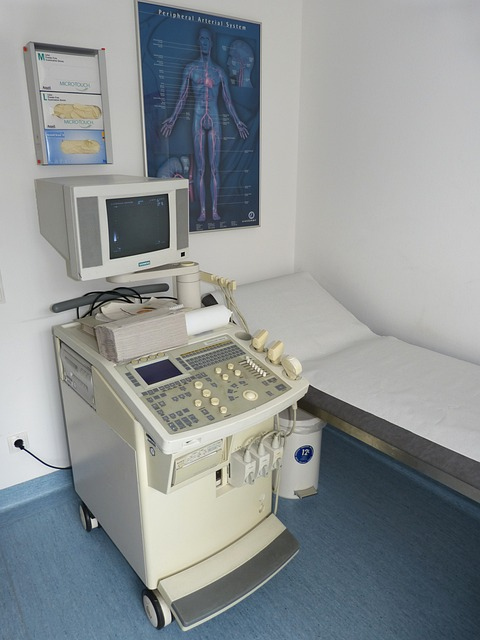
\includegraphics[width=3cm]{echographie.jpg}}
\begin{enumerate}
    \item Représenter les données sous forme d'un tableau à double entrée.
    \item Quelle est la spécificité du diagnostic de l'appendicite par échographie abdominale ?\\
    Que signifie la valeur obtenue ?
    \item Quelle est la sensibilité du diagnostic de l'appendicite par échographie abdominale ?\\
    Que signifie la valeur obtenue ?
    \item Quelle est la valeur prédictive positive du diagnostic de l'appendicite par échographie abdominale ?\\
    Que signifie la valeur obtenue ?
    \item Quelle est la valeur prédictive négative du diagnostic de l'appendicite par échographie abdominale ?\\
    Que signifie la valeur obtenue ?
\end{enumerate}

\exo{}
Lorsqu'il emprunte des livres à la bibliothèque, Mathieu en emprunte 1, 2, 3 4, ou 5 avec la même probabilité. On appelle $L$ la variable aléatoire donnant le nombre de livres empruntés par Mathieu lorsqu'il va a la bibliothèque.
\begin{enumerate}
    \item Quelle loi suit $L$ ?
    \item En déduire $E(L)$.
    \item Déterminer $P(L\geqslant 4)$.
\end{enumerate}

\exo{}
\dleft{14.5cm}{
    Pour un jeu de rôle, Sophia utilise un dé équilibré à vingt faces numérotées de 1 à 20.
    \begin{enumerate}
        \item Quelle est la loi suivie par la variable aléatoire $D$ donnant le résultat d'un lancer ?
        \item Calculer la probabilité d'obtenir une réussite critique, c'est-à-dire un 20, lors d'un lancer.
    \end{enumerate}
}
{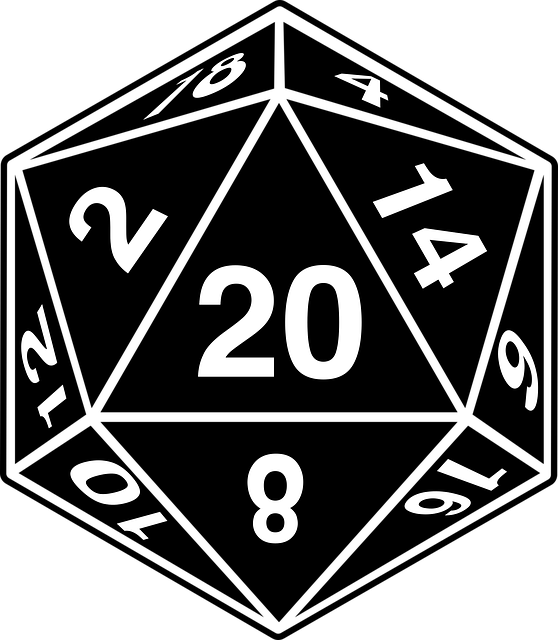
\includegraphics[width=2cm]{d20-7136921_640.png}}

\subsection*{Identifier et utiliser la loi de Bernoulli}
\exo{ Identifier une situation où une variable aléatoire suit une loi de Bernoulli}
Dans chaque cas, déterminer si la variable aléatoire $X$ suit ou non une loi de Bernoulli. Si oui, préciser le paramètre de cette loi.
\begin{enumerate}
    \item Une urne contient trois boules numérotées 0, 1 et 2. On tire une boule au hasard et on note $X$ la valeur inscrite sur la boule.
    \item On lance une pièce truquée qui a 55 \% de chances de tomber sur Pile. $X$ est la variable aléatoire qui prend la valeur 1 si la pièce tombe sur Face et 0 sinon.
    \item On lance un dé équilibré. $X$ est la variable aléatoire qui prend la valeur 1 si le résultat du lancer est supérieur ou égal à 5, et 0 sinon.
\end{enumerate}

\exo{}
Une urne contient 10 boules roses et 5 boules vertes.\\
Soit $R$ la variable aléatoire égale au nombre de boules roses obtenues (0 ou 1) lorsque l'on tire une boule au hasard dans cette urne.
\begin{enumerate}
    \item Justifier que $R$ suit la loi $\mathcal{B}\left(\dfrac{2}{3}\right)$.
    \item Combien faut-il ajouter de boules vertes dans l'urne pour que $R$ suive la loi $\mathcal{B}\left(\dfrac{1}{4}\right)$ ?
\end{enumerate}

\exo{}
Soit $X$ une variable aléatoire suivant la loi $\mathcal{B}(0,2)$.
\begin{enumerate}
    \item Donner $P(X=0)$ et $P(X=2)$.
    \item Déterminer $E(X)$.
\end{enumerate}

\subsection*{Identifier, représenter et utiliser un schéma de Bernoulli}
\exo{}
On lance trois fois successivement une pièce truquée de sorte que la probabilité d'obtenir PILE est 0,75 et on s'intéresse au nombre de PILE obtenus.
\begin{enumerate}
    \item Justifier que l'on peut associer la situation de l'énoncé à un schéma de Bernoulli dont on précisera $n$, le nombre de répétitions et $p$, la probabilité d'un succès.
    \item Représenter ce schéma de Bernoulli par un arbre.
    \item Calculer la probabilité d'obtenir exactement une fois PILE.
\end{enumerate}


\exo{}
Une entreprise estime que 5 \% des appareils qu'elle produit nécessitent un réglage au moment de la mise en service.\\
On prélève trois appareils au hasard dans la production d'une journée.
\begin{enumerate}
    \item Expliquer pourquoi on peut associer un schéma de Bernoulli à cette situation.
    \item Représenter ce schéma par un arbre pondéré.
    \item À l'aide de l'arbre, déterminer le coefficient binomial $\displaystyle \binom{3}{2}$.
    \item À l'aide de la calculatrice, déterminer le nombre de chemins comportant 14 succès dans un schéma de Bernoulli où l'on répète 20 épreuves.
\end{enumerate}

\exo{}
\begin{enumerate}
    \item Donner chacun des coefficients binomiaux suivants : $\displaystyle \binom{2}{0}, \binom{2}{2}, \binom{4}{0}, \binom{3}{3}$ et $\displaystyle \binom{5}{0}$.
    \item Même question avec $\displaystyle \binom{7}{1}, \binom{13}{1}$ et $\displaystyle\binom{81}{1}$.
    \item À l'aide du triangle de Pascal, déterminer $\displaystyle \binom{5}{2}, \binom{6}{3}, \binom{6}{4}, \binom{7}{2}$ et $\displaystyle\binom{7}{4}$.
\end{enumerate}

\subsection*{Loi binomiale}

\exo{}
On répète 10 fois de manière indépendante la même épreuve de Bernoulli de paramètre $p=0,2$.\\
Choisir la (ou les) bonne(s) réponse(s).\\
La variable aléatoire $E$ donnant le nombre d'échecs :
\begin{enumerate}[label=\ding{111}]
    \item ne suit pas une loi binomiale.
    \item suit la loi binomiale de paramètres $n=10$ et $p=0,2$.
    \item suit la loi binomiale de paramètres $n=10$ et $p=0,8$.
    \item suit la loi binomiale de paramètres $n=0,2$ et $p=10$.
\end{enumerate}


\exo{}
La ville de Las Vegas accueille environ 100 000 touristes chaque jour. On estime que 5 \% des touristes ne viennent pas à Las Vegas  pour jouer au casino.\\
On interroge au hasard 10 touristes dans la rue. On note $Y$ la variable aléatoire qui compte le nombre de touristes répondant ne pas être venus dans cette ville pour jouer.\\
Expliquer pourquoi on peut considérer que $Y$ suit une loi binomiale.\\

\exo{}
\begin{enumerate}
    \item On considère une variable aléatoire $X$ qui suit la loi binomiale de paramètres $n=20$ et $p=0,83$.\\
    Calculer l'espérance de $X$.
    \item Même question avec $Y$ suivant la loi binomiale de paramètres $n=100$ et $p=0,79$.
\end{enumerate}

\dleft{12cm}{
    \exo{}
    On considère une variable aléatoire $Z$ suivant une loi binomiale représentée par le diagramme en barres ci-contre.\\
Quelle est son espérance  ?
\begin{multicols}{4}
    \begin{enumerate}[label=\ding{111}]
        \item 8
        \item 0,26
        \item 3
        \item 6
    \end{enumerate}
\end{multicols}
}
{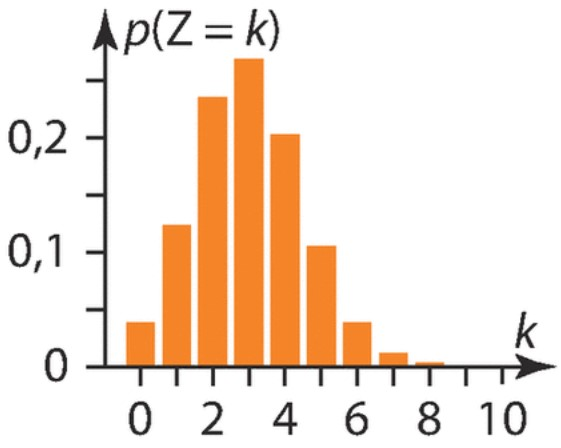
\includegraphics[width=4.5cm]{diagramme1.jpg}}


\exo{}
\dleft{12cm}{
    On donne ci-contre le diagramme en barres associé à une loi binomiale de paramètres $n=10$ et $p$ inconnu.\\
    Parmi les trois réels ci-dessous, lequel est susceptible d'être la valeur de $p$ ?
    \begin{multicols}{3}
        \begin{enumerate}[label=\ding{111}]
            \item 0,66
            \item 0,16
            \item 0,87
        \end{enumerate}
    \end{multicols}
}
{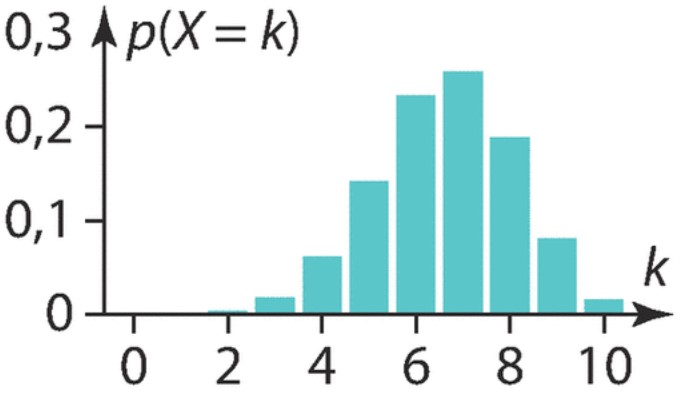
\includegraphics[width=4.5cm]{diagramme2.jpg}}


\exo{}
On considère une variable aléatoire $X$ qui suit la loi binomiale de paramètres $n=50$ et $p=0,63$.
\begin{enumerate}
    \item Déterminer le plus petit intervalle de fluctuation au seuil de 95 \% associé à $X$ de la forme $\fif{0}{b}$.
    \item Déterminer un intervalle de fluctuation centré au seuil de 95 \% associé à $X$.
\end{enumerate}

\exo{ Test d'une pièce de monaie}%Hyperbole p 217
Hugo et Aya jouent à Pile ou Face avec une pièce de monaie.\\
Au bout de plusieurs parties, lassé de perdre, Hugo prétend que la pièce n'est pas équilibrée et que la probabilité d'obtenir Face n'est pas égale à $\dfrac{1}{2}$.\\[.5em]
Pour vérifier cette affirmation, Hugo et Aya ont une idée, ils décident de langer 100 fois la pièce de monnaie et de compter le nombre de fois où ils obtiennent Face. Sur les 100 lancers, ils obtiennent 41 fois Face.

\section*{Partie A : Loi de probabilité théorique de la pièce}
On suppose que la pièce est équilibrée.\\
$X$ est la variable aléatoire qui donne le nombre d'apparitions de Face sur 100 lancers d'une pièce équilibrée.
\begin{enumerate}
    \item Quelle est la loi de probabilité de $X$ ?
    \item Calculer $E(X)$ et $\sigma(X)$.
\end{enumerate}

\section*{Partie B : À la recherche d'un intervalle}
On se propose de déterminer une intervalle $I$ de la forme $\fif{50-m}{50+m}$ tel que\\ $P(X\in I)\geqslant 1-\alpha \quad$ où $\alpha$ est un nombre réel donné de l'intervalle $\oio{0}{1}$.
\begin{enumerate}
    \item \faCalculator \hspace*{.2cm} Représenter graphiquement le la loi de probabilité de $X$ avec un diagramme en bâtons.
    \begin{enumalph}
        \item \faCalculator \hspace*{.2cm} Déterminer la plus petite valeur de $m$ telle que 
        $$P(X\in\fif{50-m}{50+m})\geqslant 0,90 \quad \text{(ici $\alpha=0,1$).}$$
        \item Conclure :\\
        Dans plus de 90 \% des échantillons de 100 lancers, la fréquence d'apparition de Face est comprise entre .......... et ..........
        \item La fréquence d'apparition de Face obtenue par Hugo et Aya appartient-elle à cet intervalle ?\\
        On dit qu'\textbf{au seuil de 90 \%, on rejette l'hypothèse que la pièce est bien équilibrée}.
    \end{enumalph}
    \item On choisit maintenant $\alpha=0,05$.
    \begin{enumalph}
        \item Déterminer le plus petit entier naturel $m$ tel que $\quad P(X\in\fif{50-m}{50+m})\geqslant 0,95$.
        \item La fréquence d'apparition de Face obtenue par Hugo et Aya appartient-elle à cet intervalle ?\\
        Compléter : Au seuil de 95 \%, on ........................................ l'hypothèse que la pièce est bien équilibrée.
    \end{enumalph}
\end{enumerate}

%\exo{ Surbooking}
%Indice page 241

\exo{ Validation d'un modèle}
On estime que dans une population donnée, 72 \% utilisent au moins un réseau social. On suppose que l'utilisation d'un réseau social par une personne donnée n'influe pas sur les autres personnes de la population étudiée. On interroge au hasard 100 personnes de cette population et on note $X$ le nombre de personnes utilisant au moins un réseau social parmi ce groupe de 100 personnes.
\begin{enumerate}
    \item Donner la loi suivie par $X$ ainsi que ses paramètres.
    \item Quelle est l'espérance de $X$ ? Interpréter ce nombre.
    \item \faCalculator \hspace*{.2cm} Déterminer le plus petit entier $k$ tel que $\quad P(X\leqslant k)\geqslant 0,95$.\\
    Interpréter ce résultat.
    \item \faCalculator \hspace*{.2cm} Donner une approximation au millième de $\quad P(65\leqslant X\leqslant 79)$.\\
    Qu'est-ce-que cela signifie pour les valeurs prises par la variable aléatoire ?
    \item Sur les 100 personnes interrogées, 77 utilisent un réseau social.\\
    Au vu des questions \textbf{3.} et \textbf{4.}, l'échantillon semble-t-il conforme aux attentes ? Avec quelle probabilité peut-on accepter ce modèle ?
\end{enumerate}

\exo{ Surbooking}%Indice p 241
\dleft{12cm}{
    Il est important pour une compagnie aérienne d'optimiser les recettes liées aux vols qu'elle assure. Certaines compagnies ont recours à la pratique de la surréservation (ou « surbooking ») et vendent plus de billets que de places dans l'avion. Le problème pour la compagnie est de ne pas non plus vendre trop de billets : cela l'amènerait à rembourser les personnes ne pouvant embarquer et nuirait à son image.\\
}
{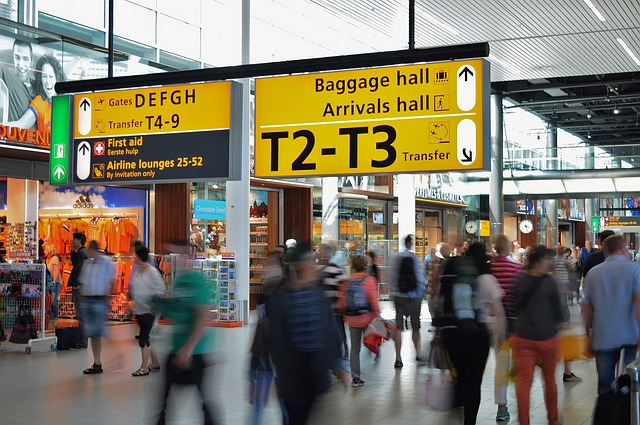
\includegraphics[width=4cm]{airport-384562_640.jpg}}

On va chercher à optimiser le taux de surréservation sans dépasser un niveau de risque raisonnable pour la compagnie « In the air ».

\section*{Partie A : Modélisation du problème}
La compagnie « In the air » dispose d'un avion de 240 places pour un vol intérieur. On considère que les comportements des passagers sont indépendants les uns des autres et on évalue à 0,9 la probabilité qu'un passager soit présent à l'embarquement. On suppose dans cette partie que la compagnie a vendu exactement 240 places et on nomme $X$ la variable aléatoire égale au nombre de passagers embarquant parmi les 240 possibles.
\begin{enumerate}
    \item Justifie que $X$ suit la loi binomiale de paramètres $n=240$ et $p=0,9$.
    \item Quelle est l'espérance de $X$ ? Interpréter ce nombre dans le contexte.
    \item Calculer $P(X\leqslant 219)$. Donner une interprétation de ce nombre expliquant la nécessité pour la compagnie d'avoir recours à la surréservation.
    \item \faCalculator \hspace*{.2cm} Déterminer le plus petit entier $k$ tel que $P(X\leqslant k)\geqslant 0,95$, puis interpréter le résultat.
\end{enumerate}

\section*{Partie B : Étude du risque de surréservation}
La compagnie a vendu 257 places alors qu'elle n'en dispose que de 240.
\begin{enumerate}
    \item Quel est le taux de surréservation, c'est-à-dire le rapport entre le nombre de places vendues au-delà de la capacité de l'appareil et cette même capacité ? On exprimera le résultat en pourcentage, arrondi à 0,1 \%.
    \item On note $Y$ la variable aléatoire égale au nombre de passagers se présentant effectivement à l'embarquement. Déterminer la loi suivie par la variable aléatoire $Y$ et en préciser les paramètres.
    \item \begin{enumalph}
        \item Pour quelles valeurs de $Y$ la compagnie devra-t-elle refuser des passagers à l'embarquement ?
        \item Déterminer la probabilité que la compagnie doive refuser au moins 1 client.
    \end{enumalph}
    \item \faCalculator \hspace*{.2cm} La compagnie souhaite ne pas prendre un risque supérieur à 1 \%. La solution envisagée est-elle acceptable pour la compagnie ? Si non, quel nombre de places maximum lui conseillez-vous de vendre pour ne pas dépasser ce risque ?
\end{enumerate}



\subsection*{Loi géométrique}

\exo{}%Indice p 2023
Dans chacun des cas suivants, déterminer si la variable aléatoire $X$ proposée suit ou non une loi géométrique. Si oui, préciser alors le paramètre de cette loi.
\begin{enumerate}
    \item Une urne contient un boule blanche et deux boules noires. On tire au hasard, successivement et avec remise, $n$ boules de cette urne. On note $X$ la variable aléatoire comptant le nombre de de boules blanches obtenues.
    \item On lance un dé équilibré à six faces plusieurs fois de suite : tant qu'on n'a pas obtenu un 6, on continue à lancer le dé. $X$ est la variable aléatoire qui compte le nombre de répétitions nécessaire à l'obtention d'un 6.
    \item Une joueuse de tennis réussit ses services 8 fois sur 10. $X$ est le nombre d'essais nécessaires pour réussir un service.
\end{enumerate}

\exo{}%Hyperbole p 203
On lance un dé équilibré jusqu'à ce qu'un 1 apparaisse pour la première fois.\\
$X$ est la variable aléatoire qui donne le nombre de lancers nécessaires pour obtenir 1.
\begin{enumerate}
    \item Déterminer la loi de probabilité de $X$.
    \item Calculer l'espérance. Interpréter le résultat obtenu.
    \item Calculer et interpréter :
    \begin{multicols}{3}
        \begin{enumalph}
            \item $P(X=3)$
            \item $P(X>5)$
            \item $P(X\leqslant5)$
        \end{enumalph}
    \end{multicols}
\end{enumerate}

\exo{}
Un couple a recours à des Fécondation In Vitro (FIV) pour avoir un enfant. Le taux moyen de succès d'une FIV est de 25 \% environ. Au-delà de 4 tentatives, les FIV ne sont plus remboursées par la Sécurité Sociale.\\
\textit{Arrondir les résultats au millième.}\\
Quelle est la probabilité pour le couple :
\begin{enumerate}
    \item De devoir faire plus de trois FIV pour avoir un enfant ?
    \item D'avoir un enfant grâce à la FIV en étant remboursé par la Sécurité Sociale ?
\end{enumerate}

\exo{}%Hyperbole p212
Dans un restaurant, on modélise le temps d'attente, en minutes, pour qu'une table se libère, par une variable aléatoire $X$ qui suit la loi géométrique de paramètre $p=0,1$.\\
\textit{Arrondir les résultats au centième.}
\begin{enumerate}
    \item Quelle est la probabilité qu'un client attende entre 5 et 10 minutes pour obtenir une table ?
    \item Un client attend depuis 10 min.\\\
    Quelle est la probabilité qu'il doive attendre au moins 5 min de plus pour obtenir une table ?
    \item Calculer $E(X)$. Interpréter le résultat obtenu.
\end{enumerate}

\exo{}
La durée de vie, en année, d'un élément radioactif peut être modélisée par une variable aléatoire $T$ qui suit la loi géométrique de paramètre $p=0,000 5$.\\
Le succès est alors l'événement « L'élément n'émet plus de rayonnement ».\\
$T$ compte le nombre d'années nécessaires pour arriver au succès. \textit{Arrondir les résultats au millième.}
\begin{enumerate}
    \item Calculer :
    \begin{multicols}{3}
        \begin{enumerate}[label=\textbullet]
            \item $P(T>3000)$
            \item $P(T\leqslant 5000)$
            \item $P(1500<T\leqslant 2500)$
        \end{enumerate}
    \end{multicols}
    \item Calculer la probabilité que cet élément ne soit pas désintégré au bout de 2000 ans sachant qu'il n'a pas été désintégré au bout de 1000 ans.
    \item La \textbf{demi-vie} d'un élément radioactif est le temps au bout duquel cet élément a une chance sur deux de ne plus émettre de rayonnement.\\
    \faCalculator \hspace*{.2cm} Déterminer la durée de demi-vie de cet élément.
\end{enumerate}

\end{document}